\section{CLoMA-UWR Framework}
\label{sec:system-design}

This section formulates multi-UAV wildfire rescue as a sequence from
fire-situation understanding to resource-constrained mission planning and
runtime replanning, and presents CLoMA-UWR as the framework that implements this
sequence. The task model represents aerial observations,
fire points, task zones, UAV operational states, mission constraints, runtime
perturbations, and the corresponding initial and revised mission plans. It
exposes three decision risks: a generated plan may violate tactical or structural
constraints, one-shot reasoning may fail to use relevant prior experience, and
an initially feasible plan may become obsolete during execution. As shown in
Figure~\ref{fig:method-overview}, Vision Analysis and Mission Planning construct
candidate plans, Validation checks them before execution, Memory supplies prior
experience, and Runtime Replanning revises the active mission after operational
state changes. The following subsections detail the task model and system
components.

\subsection{Task Modeling}

For each mission, the rescue world is represented by the structured state $S$:
\[
S=\{O,F,R,U,C,E\}.
\]
Here, $O$ denotes aerial observations; $F$ denotes fire points; $R$ denotes
task zones; $U$ denotes UAV operational states; $C$ denotes mission constraints;
and $E$ denotes runtime perturbations. This representation
separates the underlying rescue world from the information available to the
decision system. At mission start, the system receives the initial input
$X_0=\{O,U,C\}$, whereas $F$ and $R$ must be inferred from the observation. 
When a runtime perturbation occurs, it receives the updated operational 
state $U_t$ and the observed perturbation $E_t$. The required outputs are an 
initial mission plan $P$ and, when necessary, a revised plan $P'$.

The resulting task model comprises the following decision chain:
\[
\begin{gathered}
O \rightarrow F \rightarrow R,\qquad (R,U,C) \rightarrow P, \\
(P,U_t,E_t) \rightarrow P'.
\end{gathered}
\]
The first two relations transform raw aerial observations into an actionable
regional representation of the fire situation. The third relation generates an
executable fleet plan under operational constraints. The final relation adapts
that plan to changes encountered during execution. This formulation captures
the continuous rescue workflow while retaining the stage-specific information
needed to design and evaluate a closed-loop system.

\subsection{Proposed Framework}

\begin{figure*}[!t]
    \centering
    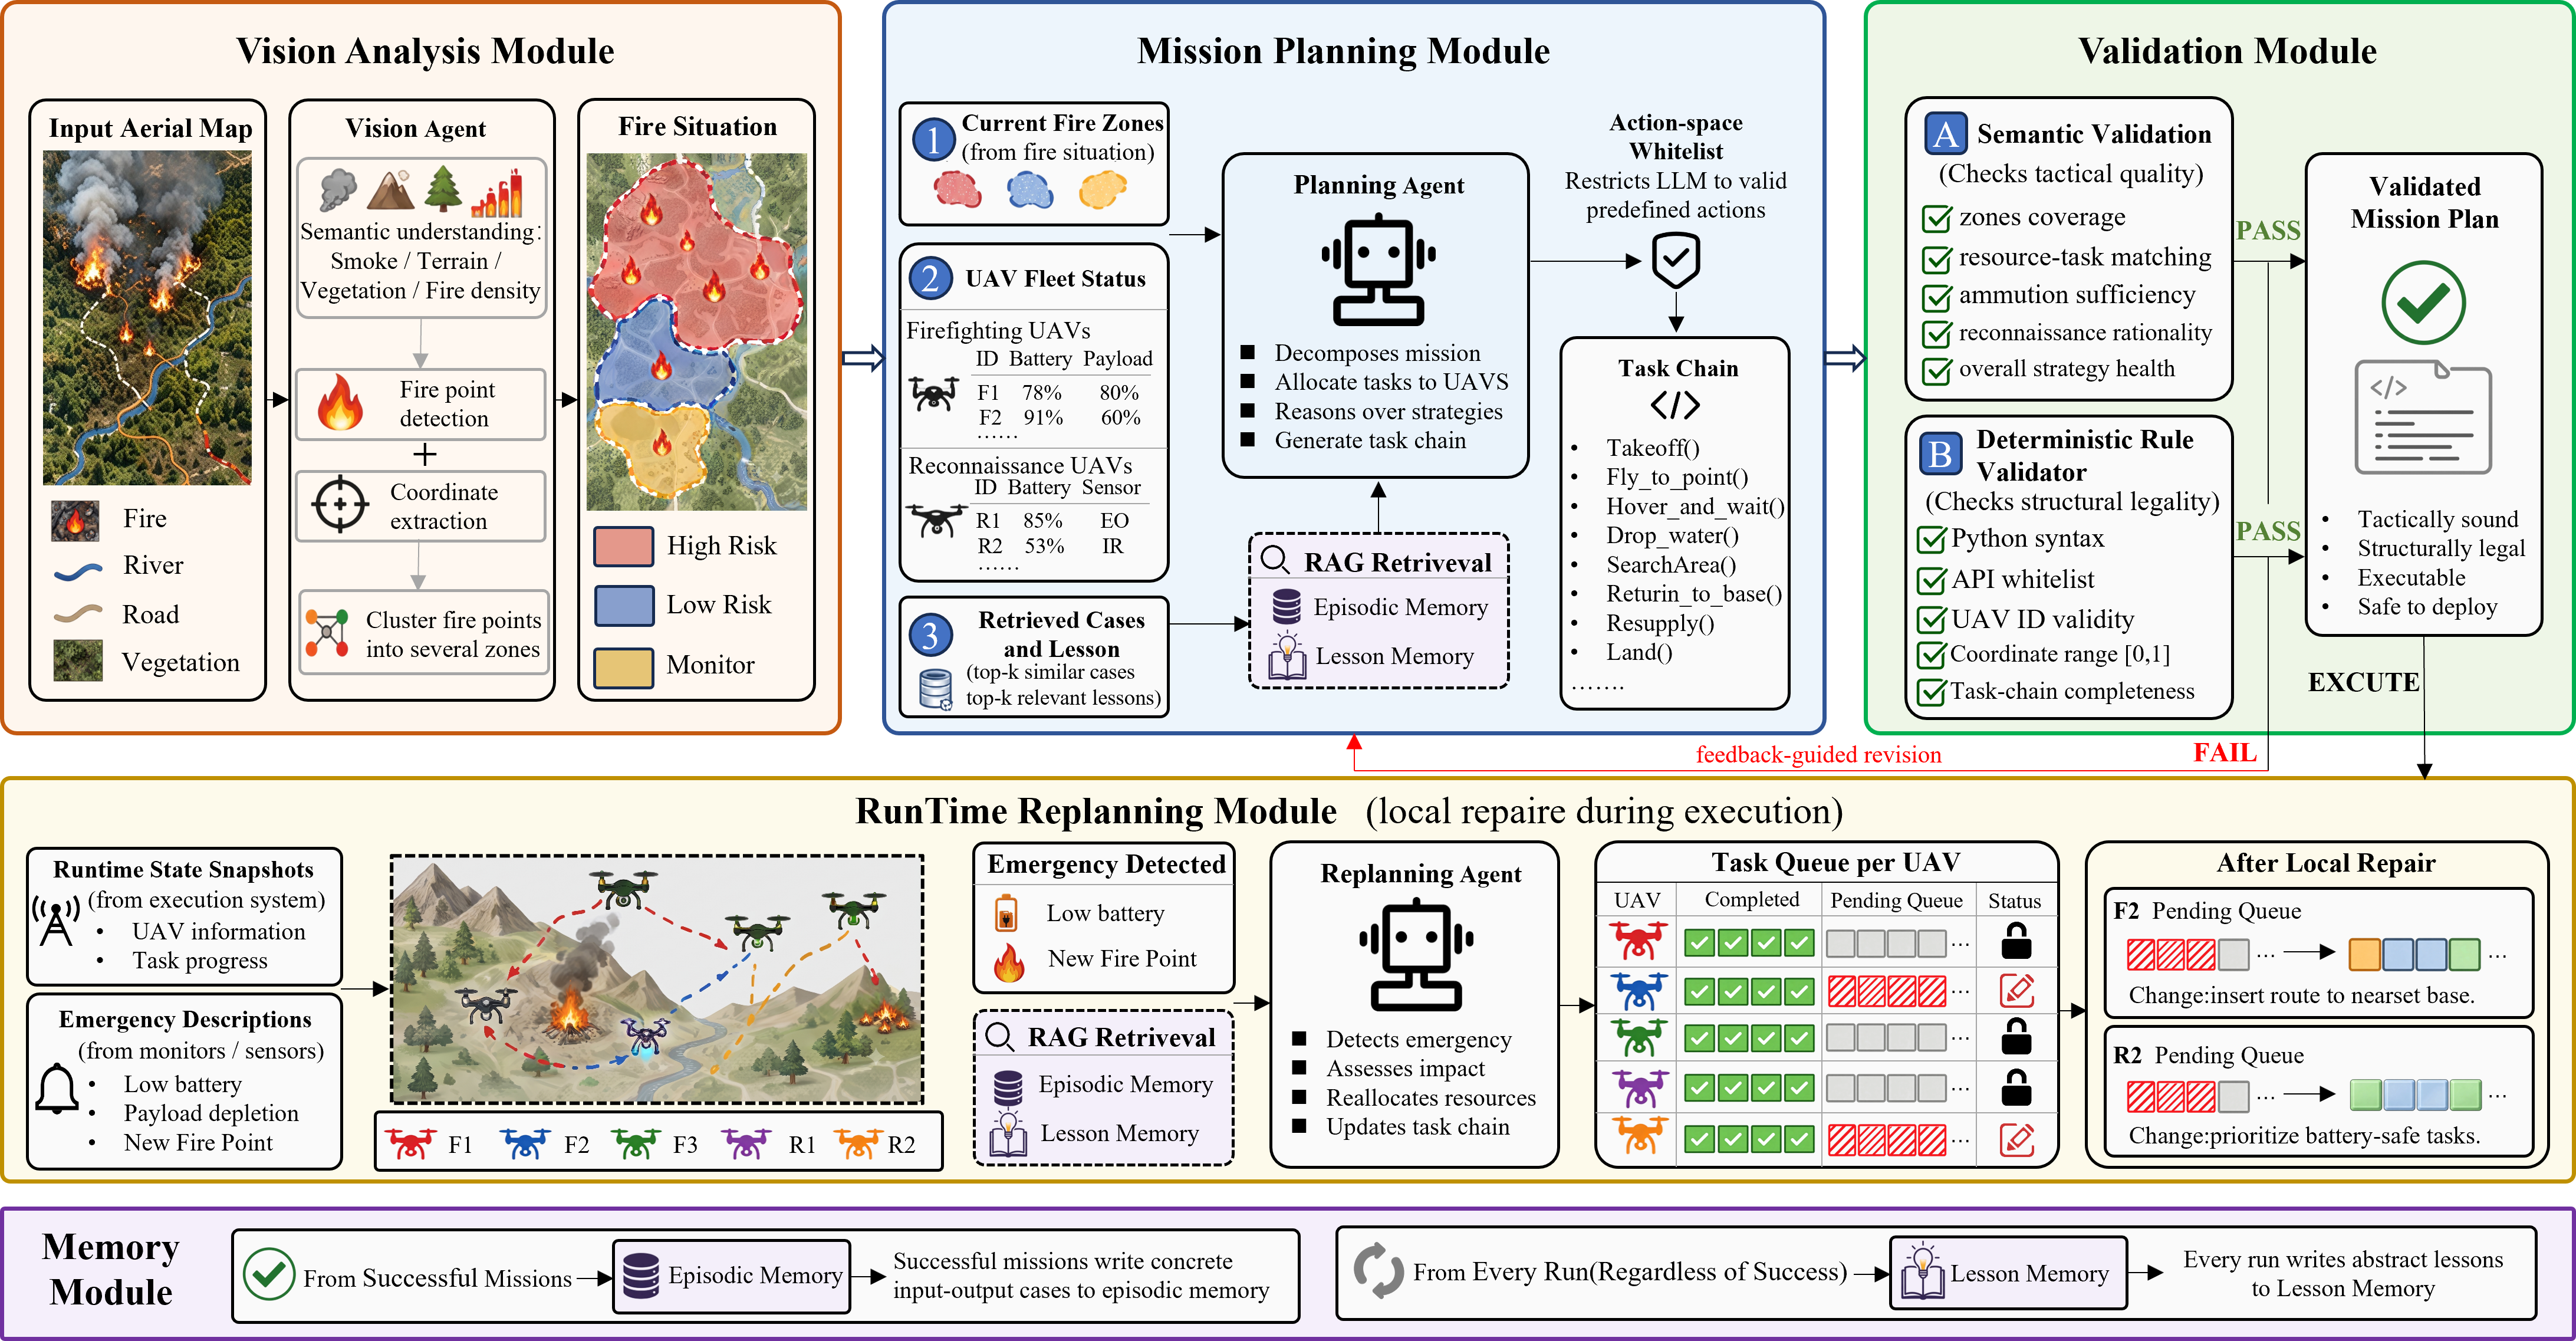
\includegraphics[width=1\textwidth]{figures/system-overview.png}
    \makeatletter
    \long\def\@makecaption#1#2{%
        \@IEEEfigurecaptionsepspace
        \hbox to\hsize{\normalfont\footnotesize\hfil
            \hbox{\normalfont\footnotesize #1.\nobreakspace\nobreakspace #2}\hfil}}
    \makeatother
    \caption{Overview of CLoMA-UWR.}
    \label{fig:method-overview}
\end{figure*}

Figure~\ref{fig:method-overview} summarizes the flow of mission state, candidate
plans, corrective feedback, and prior experience among the CLoMA-UWR components,
whose individual roles are described below.

\paragraph{Vision Analysis} Vision Analysis anchors the decision loop by
reducing the ambiguity between raw aerial observations and the planning state.
It converts raw aerial imagery into a structured description of the fire
situation.
This module uses a multimodal LLM to perform two tasks in a single inference pass.
First, it detects all visible fire points in the image and outputs their normalized coordinates.
Second, it clusters these points by spatial density, partitioning the continuous fire field
into several discrete task zones.

This module uses a multimodal LLM rather than a vision-only model because zone division
depends on more than fire point locations.
The division also depends on visual context, such as smoke, vegetation,
and terrain boundaries.
These cues require joint reasoning over appearance and spatial semantics.
The resulting fire points and task zones provide the shared initial-state
representation used by Mission Planning.

\paragraph{Mission Planning} Mission Planning addresses the fleet-level
coupling among task priorities, vehicle states, and resource constraints. It is
the core decision module and converts the structured fire situation produced by
Vision Analysis into a candidate multi-UAV collaborative plan. A planning LLM
generates a complete task chain for each UAV in the fleet, covering task
allocation, temporal sequencing, and endurance management. To keep outputs
controllable, the LLM is restricted to a predefined set of allowable actions.

Mission Planning combines the fire situation, retrieved experience,
and operational constraints.
It receives the structured fire situation from Vision Analysis,
retrieves relevant prior experience from Memory,
and produces a coordinated plan in which each UAV's task chain respects
the fleet's capabilities and the mission's operational constraints.
Formally, the planning process is expressed as
\begin{equation}
P=\mathcal{G}\bigl(R,U,C,M(q)\bigr),
\qquad q=q(R,U,C),
\label{eq:memory-augmented-planning}
\end{equation}
where $\mathcal{G}$ denotes the planning LLM, $q(R,U,C)$ denotes the query
construction from the current task zones, fleet states, and constraints, and $M(q)$ 
denotes the prior experience retrieved from Memory for that query.
The resulting $P$ is a candidate plan rather than an automatically trusted
output; it is passed to Validation before mission execution.

\paragraph{Validation} Validation addresses the risk that a linguistically
coherent candidate plan may still be tactically implausible or structurally
invalid. It evaluates tactical rationality and structural legality, including
zone coverage completeness, resource-task matching, payload adequacy, UAV
existence, coordinate validity, and task-chain completeness. When Validation
rejects a plan, its feedback is routed back to Mission Planning as targeted
guidance for revision. Only an accepted plan proceeds to execution, preserving
the separation between plan generation and plan acceptance.


\paragraph{Runtime Replanning} Runtime Replanning addresses the risk that an
accepted plan becomes invalid after the operational state changes. This module
handles runtime perturbations during mission execution.
It takes a runtime state snapshot as input, including current positions, battery levels,
payloads, and task progress for each UAV.
Its output is not a new global plan, but a local revision of the current plan.
Unlike the main pipeline, Runtime Replanning reasons about a dynamic execution state and
changes only the affected part of the plan.

When a runtime perturbation occurs, the module retrieves similar prior cases
from Memory as repair references.
These cases describe how comparable failures were resolved in past missions,
providing the replanning LLM with tactical precedents for the current situation.
The resulting local revision closes the execution-feedback loop without
restarting the complete pre-execution pipeline.

\paragraph{Memory} Memory addresses the risk that relevant prior experience is
unavailable when coupled resource, scheduling, or event conditions make the
current decision less routine. It allows the system to reuse past experience.
Each memory entry records a task situation, the generated or revised plan,
validation feedback, runtime perturbations, the execution outcome, and reusable
guidance extracted from the completed mission. Memory is represented as
\begin{equation}
M=\{(z_i,P_i,o_i)\}_{i=1}^{N},
\label{eq:memory-store}
\end{equation}
where $m_i=(z_i,P_i,o_i)$ denotes a memory entry, and $z_i$, $P_i$, and
$o_i$ denote the task situation, the associated plan, and the execution outcome
of completed mission $i$, respectively. Validation feedback, runtime perturbations, 
and reusable guidance are retained as associated information. The system retrieves 
the $K$ most semantically similar entries to the current query according to
\begin{equation}
\begin{aligned}
\mathcal{R}_K(q,M)
&=\underset{m_i\in M}{\operatorname{TopK}}\;
  \operatorname{sim}(q,m_i),\\
\operatorname{sim}(q,m_i)
&=\frac{\phi(q)^\top\phi(m_i)}
{\lVert\phi(q)\rVert_2\lVert\phi(m_i)\rVert_2}.
\end{aligned}
\label{eq:semantic-memory-retrieval}
\end{equation}
where $\mathcal{R}_K(q,M)$ is the set of the $K$ entries retrieved from $M$ for
query $q$, $\phi(\cdot)$ maps a query or memory entry to its semantic embedding. 
The retrieved set provides Mission Planning or Runtime Replanning with concrete 
tacticalprecedents and reusable guidance about recurring planning, resource-management,
and repair patterns.

\endinput
